\chapter{Background}\label{ch:02background}

In this chapter, some of the theoretical background information required for this thesis is examined. An overview of experimental evolution is given before moving on to a discussion of Aevol, the specific tool that was used in this thesis. The chapter closes examining how Aevol can be used to study reductive evolution and by discussing the current state of the literature surrounding reductive evolution.  

\section{Properties of Genomes}
This section describes some general properties of evolutionary theory which will be required for this thesis. Some general properties about evolution were covered in Section~\ref{ch:01intro} and now some more specific properties of genomes will be examined, as these will play a large role in the coming experiments. 

\subsection{Evolvability}\label{subsec:evolvability}
Evolvability is usually defined as the ``prospective ability [of a population] to produce new mutations that can be used in adaptive evolution in the medium to long term'' \cite{brookfield2009evolution}. In other words, a system has evolvability if ``mutations in it can produce heritable phenotypic variation''\cite{doi:10.1098/rspb.2007.1137} and, critically, that this is not simply having a large amount of genetic diversity but rather \textit{adaptive} diversity which provides some benefit. 

There is, then, a link between evolvability and selection, since it is of course in an organism's best interest to be able to adapt to new environments or situations. Evolvability should, therefore, be selected for, though it may not be obvious how, say, a random mutation which confers no immediate benefit (but which increases evolvability) may be selected for. One possibility might be the idea of ``genetic hitchhiking'', in which an allele changes its frequency not because it is itself under selection but because it is near another gene which \textit{is} under selection. Intuitively, if an ``evolvability trait'' arises which provides no immediate fitness benefit but which confers some benefit to offspring, eventually this trait will also increase in frequency as the fitness advantage conferred on the offspring causes them to be selected. The idea is discussed at greater length by Arenas et al.~\cite{selectionEvolvability}. 

In real-world scenarios, it can be difficult to calculate evolvability for two reasons. First, evolvability can usually only be measured over evolutionary timescales. It isn't usually possible to look at a genome and determine its evolvability, since this involves looking at its offspring and examining their fitness (or some other phenotype) in some environment. Second, the stochastic nature of mutations makes it very difficult in real-world scenarios to compare two populations, since one has to separate the noise of random mutations from the signal of evolvability~\cite{selectionEvolvability}. 

\subsection{Robustness and Antirobustness}\label{subsec:robustness_antirobustness}
Robustness is broadly defined as the ability of an organism to withstand disruptions or perturbations without affecting its phenotype. There are differing kinds of robustness, as well: one may describe robustness in terms of mutational robustness\textendash which describes the extent to which an organism's phenotype is not affected by stochastic mutational events\textendash or one may speak of environmental robustness, which describes the ability of an organism to maintain its phenotype in diverse environments with little or no loss in fitness. 

Also important is the idea of antirobustness, wherein an organism may actually \textit{thrive} on such perturbations. This has been suggested as a possible method of minimizing the effects of \textit{Muller's ratchet}, wherein deleterious mutations accumulate in a population as a result of genetic drift\cite{Gordo2137}. A large number of initially-deleterious mutations may provide fodder for selection to fix more beneficial mutations in the population\cite{doi:10.1186/s12862-019-1507-z}.

There is, then, a seeming trade-off between robustness and evolvability. The more robust a system is, the less phenotypic variation is generated by random mutation events, and thus less evolvability. However, a key factor is to distinguish between genomic and phenotypic robustness; a strong phenotypic robustness promotes structural evolvability, as the likelihood that a mutation is deleterious is smaller in populations with more robust phenotypes. For a fuller discussion, see Wagner et al.~\cite{doi:10.1098/rspb.2007.1137}.

\subsection{Fitness}\label{background:fitness}
In population genetics, ``fitness'' can relate to either the genotype or the phenotype and denotes the contribution of an individual to the gene pool of the next generation; it is usually discussed in terms of \textit{absolute fitness} and \textit{relative fitness}~\cite{cutter2019primer}. The absolute fitness $W$ of a genotype is the level of proportional change in the abundance of that genotype from one generation to the next. So if, for example, a genotype in generation $t$ exists with abundance $n(t)$, then $n(t+1) = W*n(t)$. 

Relative fitness, on the other hand, describes the change in genotype \textit{frequency}, i.e. the fraction of all chromosomes in the population that carry a particular allele. For a population of size $N$, if a genotype's frequency at time $t$ is given by $p(t) = n(t)/N(t)$, then $p(t+1) = \frac{w}{\bar{w}}*p(t)$, where $\bar{w}$ is the mean relative fitness in the population. This implies that $\frac{w}{\bar{w}}$ is proportional to $\frac{W}{\bar{W}}$. 

\section{Reductive Evolution}\label{reductive_evolution}
Reductive evolution is the process by which organisms evolve to have a smaller average genome size than their ancestors via a pattern of gene loss~\cite{wilcox2003consequences}. This has been observed both in free-living bacteria such as \textit{Prochlorococcus} as well as endosymbiotic bacteria living inside host cells (e.g. \textit{Buchnera aphidicola} in aphids). Patterns consistent across most cases of reductive evolution are: a reduced GC content (impacting protein stability), gene loss, low non-coding to coding DNA ratios, and rapid sequence evolution~\cite{Batut.2014}. Some of the hypothesized mechanisms behind reductive evolution include: limits imposed by the effective population size (i.e. ``Muller's ratchet'', described below), the ``Black Queen Hypothesis'', and environmental adaptation. 

In Muller's ratchet, organisms with smaller effective population sizes, such as \textit{Buchnera aphidicola}, may lose genes because deleterious mutations accumulate in a population due to the smaller population size not allowing for enough variability. In the absence of recombination, these deleterious mutations become fixed in a population. The idea was originally put forth by H.J. Muller~\cite{MullersRatchet}.

The Black Queen Hypothesis suggests that genes may be lost when some subset of the bacteria in a community is able to provide the same function as the lost genes for the benefit of the rest of the community, allowing some bacteria to lose those genes and receive the benefit from others~\cite{morris2012black}. 

Lastly, one other proposed hypothesis among many has been environmental adaptation. For example, many reduced strains of the marine cyanobacteria \textit{Prochlorococcus} live in nutritionally-poor surface waters. It has been suggested that perhaps genome reduction is an adaptation which allows reduced strains to conserve precious nutrients~\cite{rocap2003genome, dufresne2005accelerated}. 

\section{Experimental Evolution}
As discussed in Chapter~\ref{ch:01intro}, in vivo experiments, although sometimes more realistic, have their own set of difficulties. Some examples of these difficulties include recreating challenging environmental conditions (e.g. simulating the open ocean in a laboratory) and identifying and/or simulating the multiple selection pressures acting on genomes in the real world~\cite{Batut.2013}. These challenges add enormous difficulty and complexity to conducting proper experiments and isolating the specific factors which lead to particular outcomes. 

In silico evolution simulates the evolution of organisms in software, thus allowing for far greater control and analysis of the environment and other experimental conditions. In contrast to in vivo experiments, a greater amount of control is also available with regard to the way organisms may interact, reproduce, and evolve. For example, a genome may be created completely from scratch or an existing genome may be fed into the simulation. Reproduction rates can depend on overall fitness, on relative fitness, or some other criterion. 

Factors such as the mutation rates or selection pressure are then parameters for the model and may be kept constant or allowed to vary over time. Given that these are parameters of the system, they may be tightly controlled, leading to a clearer picture of the factors influencing different outcomes. An underlying deterministic model can also allow for a reconstruction of the system from any given point, allowing one to easily create a record of events, including phylogenetic trees. 

Although there are certainly limitations to using in silico evolution (see Section~\ref{limitations}), overall in silico experimental evolution is a valuable tool for studying the underlying mechanisms of evolution when real-world experiments would be prohibitively time-consuming or expensive.

Many silico evolution tools have been used to test various aspects of evolution, and several formalisms exist to represent the process. In a ``sequence-of-nucleotides'' model, genomes are represented by a string of characters representing base pairs. Other formalisms include the ``gene network model'' in which genes are nodes in a connected graph, as well as the ``digital organisms'' model, in which software programs representing organisms fight for CPU time. Examples of the latter type include Tierra~\cite{Tierra-Ray} and Avida~\cite{Avida-Ofria}, which were some of the first in silico evolution tools. DOSE, an ecology-conscious method of checking for heterozygosity (variation within a population)~\cite{Castillo-DOSE} is a more recent example of in silico experimental evolution. For a more comprehensive review, see~\cite{Mozhayskiy-In-Silico-Review}. 
 
\section{Aevol}
Aevol follows a ``sequence-of-nucleotides'' model~\cite{Batut.2013} in which organisms are simulated with a binary genome which can either be generated at random or input as a previously-generated sequence. Aevol essentially consists of a repeated iteration of three main steps: 1) decoding the genome of these organisms to produce artificial proteins, 2) selecting the most fit individuals and 3) reproduction of these fittest individuals with possible variations (mutations, rearrangements, etc.). The sections below examine each of these steps in greater detail.

\subsection{Why use Aevol}

The in silico tool Aevol was developed to ``study the evolution of the size and organization of bacterial genomes in various scenarios''\cite{Batut.2013}. The program has also been expanded upon and tested in a variety of scenarios over the years (e.g. \cite{parsons2011selection}, \cite{misevic2012effects}, \cite{Miramontes.2016}). Some examples of experiments in which Aevol was the primary mechanism of in silico experimental evolution include: testing the predictability of evolution with high mutation rates as in viruses~\cite{beslon:hal-01577115}, determining whether selection is able to overcome evolution's drive towards more complex organisms~\cite{Liard.2018}, examining the role of mutators in reorganizing the genome in order to overcome mutational load~\cite{doi:10.1186/s12862-019-1507-z}, examining the effects of population shape on levels of cooperation~\cite{Miramontes.2016}, modeling regulatory networks~\cite{sanchezdehesa:hal-01502737} and more. 

As an in silico experimental evolution tool, Aevol embodies several of the advantages of in silico evolution in general. There is a ``fossil record'' of each generation, experimental conditions are tightly controlled, and experiments are easily repeatable. The encoding/decoding strategy of Aevol follows a biologically realistic model, in the sense that there are many degrees of freedom between an organism's genome and its proteome. Many genes may encode for very simple proteins (e.g. if the genes contain the same or similar sequences), and by contrast, overlapping genes may code for complex proteomes.

In the following sections, the in silico experimental evolution tool Aevol will be examined in greater detail. 

\subsection{Aevol's Architecture}
Aevol's three main steps\textemdash decoding the genome, selection, and reproduction\textemdash are illustrated in Figure~\ref{fig:aevol_overview01} and are discussed in greater detail in the following sections. 

\begin{figure}[H]
	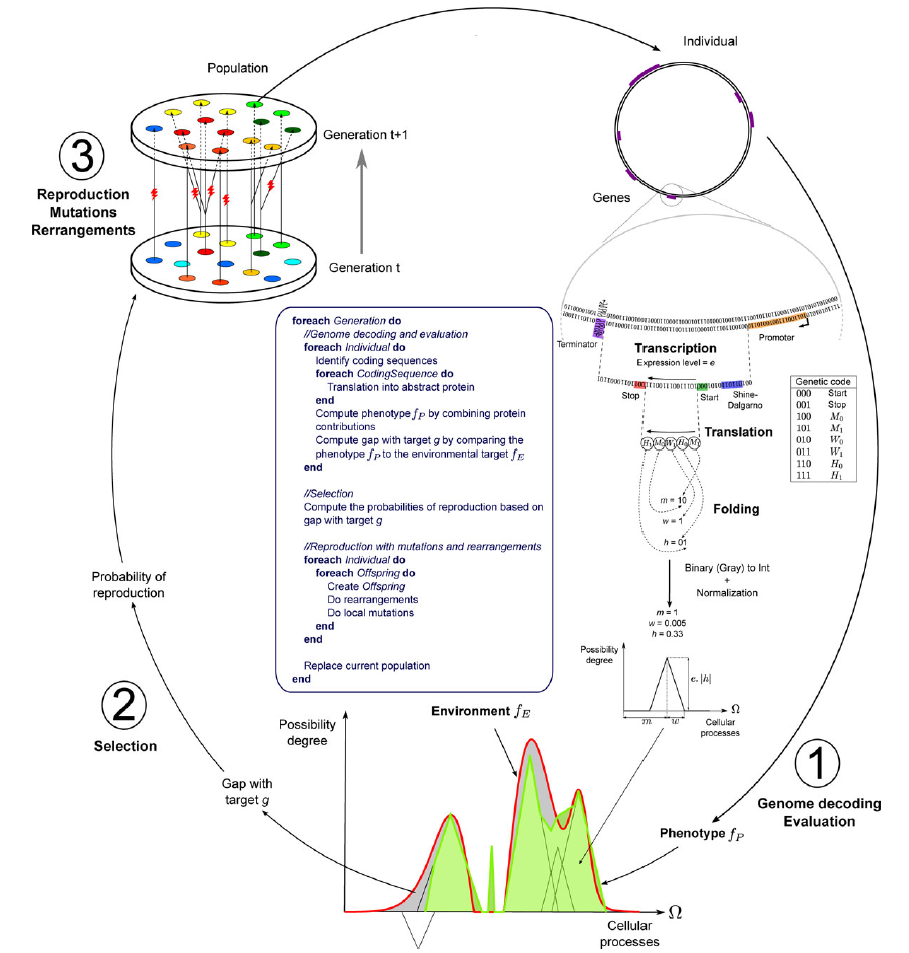
\includegraphics[width=\textwidth,height=\textheight,keepaspectratio]{aevol_overview01}
	\centering
	\caption[Overview of Aevol's architecture.]{Overview of Aevol's architecture, from~\cite{Batut.2013}. In step 1, the binary genome of the organisms is decoded and the resulting phenotype (bottom, in green) is matched up against an environmental target function (red line). In step 2, the probability of reproduction is calculated for each organism, based on its fitness (gap between the environment $f_E$ and its phenotype). In step 3, the next generation is created based on the probabilities from step 2, along with random mutations, rearrangements, etc.}
	\label{fig:aevol_overview01}
\end{figure}
\subsubsection{Decoding the Genome}\label{subsec:aevol_decoding}
In Aevol, a genome consists of a string of binary characters where 0 is complementary to 1. Each organism in the population has a double-stranded circular genome which is either generated randomly or which was provided as input. To decode the genome and produce the phenotype, the sequence is searched for transcribed regions. Transcribed regions are denoted by promoter and terminator sequences. The promoter sequence is a sequence whose Hamming distance $d$ is within $d_{max} = 4$ mismatches of the predefined consensus sequence $0101011001110010010110$. Terminators are sequences which can form a stem-loop structure with a stem size of 4 bases and a loop length of 3 bases (i.e. $abcd$***$\overline{dcba}$ where a is complementary to $\overline{a}$, b is complementary to $\overline{b}$, etc.). Lastly, the initiation and termination signals are sought, which are simply Shine-Dalgarno-like signals (i.e. $011011****000$ to start and $011011****001$ to stop). Lastly, an expression level $e$ is assigned to each coding region, following the formula $e = 1 - \frac{d}{d_{max} + 1}$ where $d$ is again the Hamming distance between the coding region and the consensus sequence given above and $d_{max}$ is the maximum allowable distance (i.e. 4). 

Once an initiation sequence is found, the following bases are read three at a time (codon by codon) until a stop codon (by default $001$) is found. If a stop codon is not found, then no protein is produced. Since a transcribed region may have multiple initiation signals, operons are therefore allowed. The codons following an initiation signal encode for three parameters according to the genetic code given in Figure~\ref{fig:aevol_overview01}: $m$ (mean), $w$ (half-width), and $h$ (height), which together define a triangle representing a ``cellular process''.

A cellular process is simply an abstract representation of some phenotypic function and is represented by the ordered set $\Omega = \left[ a,b \right] \subset \mathbb{R}$. Together, these cellular processes make up the organism's proteome. To keep things simple, $\Omega$ is a one-dimensional space in the interval $\left[0,1\right]$, i.e. a ``cellular process'' is simply a real number, and the genomic encoding of each cellular process determines the function $f(x) : \Omega \rightarrow \left[0,1\right]$. The mean $m$ gives us the specific cellular process in the range $\left[0,1\right]$. The width $w$ describes the ``scope'' of the process, i.e. the \textit{pleiotropy} of the process, meaning the subset of the protein that is in the interval $ \left(m - w, m + w\right) \subset \Omega$ . The height determines the degree of possibility of the process, i.e. its relative strength.

The codons are read one after the other and their Gray codes\footnote{A binary encoding such that two successive values (e.g. 2, 3) only differ by at most one bit (e.g. 0011, 0010). See \cite{doran2007gray} for an overview.} are used to compute the real numbers $m$, $w$, and $h$ as follows. Each parameter ($m$, $w$, $h$) is assigned two codons in the genetic code (see Figure \ref{fig:aevol_overview01}), for example $w_0 = 010$ and $w_1 = 011$. Any $w_0$ codons become a $0$ in the Gray code, and vice versa with $1$s. So if, for example, when reading the coding sequence, the codons $w_1$, $w_0$, $w_1$, $w_0$ are read, the Gray code becomes $1010$, which is 12 in decimal. This is done for $m$, $w$, and $h$, and the resulting values are then normalized to be in the proper range. $w$'s range is specified in the parameter file (as \texttt{MAX\_TRIANGLE\_WIDTH}), $h$ must be in the range $\left[-1,+1\right]$ (indicating that both activating and inhibiting processes are allowed) and $m$ must be in the range $\left[0,1\right]$ (the range of $\Omega$). 

Given the fact that there are likely multiple coding sequences in a genome, several triangles (cellular processes) are translated from the genome, each parameterized by its own $m$, $w$, and $h$. These triangles form the phenotypic function $f_P$. \textit{Fuzzy logic} is used to find the overall contribution of each cellular process, using the Lukasiewicz fuzzy operators\footnote{See \url{https://en.wikipedia.org/wiki/Lukasiewicz\_logic} for an introduction.}. Roughly speaking, the activating proteins are added up, as are the inhibiting proteins, and the difference between these two totals represents the final function $f_P$. More formally, if $f_i$ is the possibility distribution of the $i$-th activator protein and $f_j$ is the possibility distribution of the $j$-th inhibitor protein, then the phenotype of the individual is defined as:
\begin{equation*}
f_P = max\left(min\left(\sum_{i}^{}f_i(x),1 \right) - min\left(\sum_{j}^{}f_j(x),1 \right) ,0\right)
\end{equation*}

\subsubsection{Selection}\label{subsec:aevol_selection}
After the genome is decoded, the organisms are tested for their fitness. Fitness in Aevol is related to the gap between the phenotype of a sequence $f_P$ and the environmental  target function $f_E$, as illustrated in Figure \ref{fig:aevol_overview01}. This environmental target function $f_E$ is a user-defined set of Gaussians which are specified in a parameter file, with each Gaussian being identified by three parameters: its height, its location along the axis, and its width. The difference between the phenotype (as calculated above) and the environmental function is the ``metabolic error'', labeled $g$ in the figure and is more formally defined as:  $g = \int_{a}^{b} f_E(x) - f_P(x) dx$. The idea is illustrated in Figure~\ref{fig:aevol_fitness01}

\begin{figure}[H]
	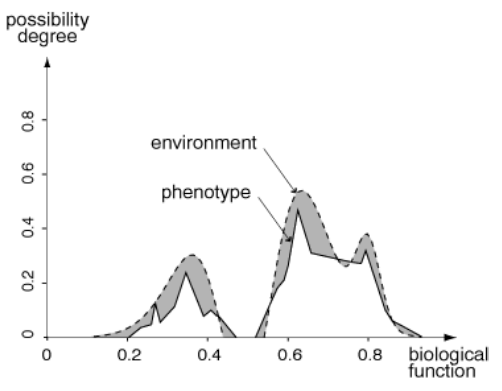
\includegraphics[scale=0.5]{aevol_fitness_description01}
	\centering
	\caption[Overview of Aevol's concept of fitness.]{Overview of Aevol's conception of fitness, from \cite{knibbe:tel-00482375}}
	\label{fig:aevol_fitness01}
\end{figure}

Aevol contains several selection schemes, but here only the \texttt{fitness\_proportionate} scheme will be considered, since this was the only selection scheme employed in these experiments. In this scheme, the probability of reproduction for each organism $i$ is proportionate to its fitness, namely:
\begin{equation*}
P(\text{reproduction}) = \frac{e^{-k * g}}{\sum_{i=1}^{N} e^{-k * g_i}}
\end{equation*} 
where $k$ is a user-definable parameter which determines the selection intensity and $g$ is the metabolic error.
\subsubsection{Reproduction}\label{subsec:aevol_reproduction}
Once the fittest organisms in the population are found and their probabilities of reproducing are calculated as described in the previous Section, new organisms are produced. This is done for each potential parent organism by drawing from a multinomial distribution with the probability of reproduction given above. The population size $N$ is kept constant and a record of each generation is kept so that the phylogenetic lineages can be recreated. Since the population size is held constant, this implies that a single organism with a high probability of reproduction may produce multiple offspring and an organism with low probability of reproduction may produce none.

When new organisms are created and their genomes are copied from their parent organisms, it is at this stage that some of the driving forces in evolution occur, namely the possibility for variation through mutation, indels, and frameshifts. Offspring will receive their parents' genome but their genome may be subject to perturbations due to stochastic effects. Mutation rates are set in the parameter file and include point mutations, insertions and deletions (indels), and rearrangements (duplication, deletions, translocations, and inversions).

The mutation, indels, rearrangement, etc. events are carried out by first determining the number $\mu$ of such events which will occur, based on the mutation rate specified in the parameter file and drawing from a binomial distribution (e.g. $B(L, \mu_\text{point})$ for point mutations, $B(L, \mu_\text{large deletions})$ for large deletions, etc. where $L$ is the size of the genome). Then a random point (or points, in the case of e.g. rearrangement) is chosen and the event is carried out, with the order of these events shuffled randomly. 

\section{Analyzing with Aevol}\label{sec:aevol_analysis}

Once the experiments have completed, Aevol by default produces several statistics files which include information about genome size, the percentage of coding DNA, number of genes, average metabolic error, and many other statistics. It further includes a number of post-treatments that allow one to analyze specific individuals or the population at large, including tools for determining robustness, evolvability, coalescence, and the lineages. 

One of the key features of Aevol is the ability to look back in time at the ''archaeological record'' of previous organisms, which is stored on disk, in order to perform various analyses. This is primarily done with a myriad of post-treatments'', i.e. supplementary programs. These post-treatments generally require a \texttt{lineage} file, which is a file generated by Aevol that shows a record back in time of the line of descent for an individual. One may specify either the best-ranked individual (i.e. the fittest) or a specific individual by their unique identification number. The basic idea is illustrated below in Figure~\ref{fig:lineage01}. 

\begin{figure}[H]
	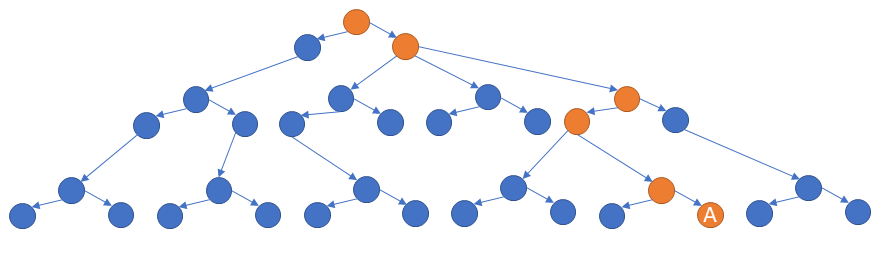
\includegraphics[width=\linewidth]{lineage01}
	\centering
	\caption[Lineage basic illustration.]{A basic illustration of a lineage. The ancestors of the individual (labeled `A') can be traced back through the previous generations for all of its ancestors (all in orange).}
	\label{fig:lineage01}
\end{figure}


\section{Related Work}\label{related_work}

%TODO Add population aspect of in silico experimental evolution - waiting on clarification from Berenice 5/20/2020 - Update 5/26/2020 never got a response. Turning it in as is. 

Much work has already been done in the field of reductive evolution and in silico experimentation, and this section will look at the current state of the literature. 

\subsection{Reductive Evolution}\label{related_work:reductive_evolution}
Regarding the influence of selection on reductive evolution, Liard et al. showed in~\cite{Liard.2018} that selection for fitness is not necessarily enough to overcome the tendency of organisms to become more and more complex. They describe the existence of a ``complexity ratchet,'' which characterizes this tendency of organisms to increase their complexity as being irreversible once the organisms have reached a certain complexity level. In their words:
\begin{quote}
	``Since gene deletion is obviously deleterious $\left[\text{in this scenario}\right]$, the only available evolutionary path for already complex organisms is a headlong rush toward increasing complexity by acquiring new genes. Hence the ratchet clicks, further widening the fitness valley that separates the current genome from a simple one, soon making it so wide it is very unlikely to be crossed."
\end{quote} 
Echoing the findings of Knibbe et al.~\cite{Knibbe2007} and performing in silico experiments with Aevol they found, however, that limiting \textit{robustness} can overcome the tendency of organisms to become more and more complex, because this places an upper bound on the amount of information that an organism can transmit in its genome. Limiting robustness by increasing the mutation rate forced gene elimination despite the fitness loss because it lowered the information content of the genome. A mutation rate of even $\mu = 10^{-4}$ resulted in nearly 40\% of their organisms developing a simpler genome.

Batut et al.~\cite{Batut.2014} investigated many of the different hypotheses which seek to explain the mechanisms behind reductive evolution (some of which were discussed in Section~\ref{reductive_evolution}), as evidenced in the marine cyanobacteria \textit{Prochlorococcus}. Among these explanations are: limits imposed by population size and ``Muller's ratchet,'' high mutation rates, the ``Black Queen Hypothesis'', and environmental adaptation. Batut et al. found that generally Muller's ratchet could explain the reduced genome size in endosymbiotic bacteria but that it was not enough to explain the reduction seen in \textit{Prochlorococcus} due to its large effective population size\textemdash some strains of \textit{Prochlorococcus} are estimated to have effective population sizes of up to $10^9$.  

Regarding the ``Black Queen Hypothesis,'' in which members of a (bacterial) community are able to reduce their genome size because other members of a community provide the lost functionality, Batut et al. found that this hypothesis was difficult to test for but suggest it may be a useful explanation for the evolution of endosymbiotic consortia.  

Given the previous discussion on high mutation rates and their impact on limiting robustness (and thus complexity), a discussion and focus on the last criterion of Batut et al., environmental adaptation, closes this section. Given the nutrient-poor environmental conditions in which \textit{Prochlorococcus} is often found, it has been suggested that perhaps the loss of genes is adaptive, since any superfluous genes (such as those required to ``respond to variation in nutrient concentrations'') inherently carry a fitness cost. However, several gene losses observed in \textit{Prochlorococcus} suggest that the reduction was not adaptive, however. For example, many DNA repair genes were lost, and the immediate fitness benefits of such a loss are not obvious. 

Regarding genome structure, in the same experiments mentioned above, Knibbe et al.\cite{Knibbe2007} also found, via in silico experimentation, that the accumulation of non-coding DNA strongly depends on the mutation rate. This in turn affects the selection trade-off between reliably passing on the existing genome and having the mutational variability to adapt to new challenges.  Under higher mutation rates, their organisms closely resembled viral genomes in that they had almost no non-coding sequences. When the selection strength was larger, genomes were larger.  Another aspect of genome structure, namely gene density, was examined by Kuo et al. \cite{kuo2009consequences}, who examined the role of genetic drift on gene density (i.e. the ratio of the number of genes per number of base pairs) and found that, as the ratio of non-synonymous to synonymous substitutions increased, gene density varied much more greatly.
\subsection{Investigations in Experimental Evolution}

Koskiniemi et al.~\cite{koskiniemi2012} performed in vivo experiments on the bacterium \textit{Salmonella enterica} in which the effects on fitness of random deletions was measured. Some 25\% of the deletions actually caused an increase in fitness under some conditions, suggesting that there is a certain cost associated with having superfluous genes and thus gene loss may be selected for under certain conditions. In the usual race between the gene-preserving force of selection and the natural tendency of bacterial genomes towards deletion and streamlining, Koskiniemi suggests that perhaps it is sometimes a team effort. 

Liard et al. showed in their experiments with Aevol that complexity can arise in organisms in even the most simple of environments (a single triangular target function) and with the most basic beginnings (a single gene and protein)~\cite{Liard.2018}. They found that the complexity continues to increase, even when the resulting organisms are much less fit than the simpler ones, and that this complexity even overcomes selection. They also found that whether an organism would develop into a simple or complex organism was usually determined quite early in its evolution, around generation 10,000. Reasoning that genome compactness is a direct driver of mutational robustness, as Knibbe et al.~\cite{Knibbe2007} showed, and that more robust organisms can be selected over fitter organisms under heavy mutational stress as shown by Wilke et al.~\cite{wilke2001evolution}, they wondered if robustness could select for a more simplified genome. To test this, they changed the mutation rate to be exceptionally high (up to $\mu = 1e^{-4} *bp^{-1}*gen^{-1}$) and ran their simulations for another 100,000 generations, and the results confirmed their expectations: The higher the differential between the old and the new mutation rate, the larger percentage of organisms evolved a more reduced genome (up to 91\% in the case of a change from $\mu_\text{old}=1e^{-6}$ to $\mu_\text{new}=1e^{-3}$).

\section{Summary}
Connecting it all together, there is, then, a natural link between the amount of non-coding DNA, coding DNA, genome size, evolvability, robustness, and selection. As the amount of non-coding bases (and often therefore overall genome size) increases through natural mutational processes, these non-coding bases can nevertheless play a crucial role in increasing evolvability by being the fodder for new potentially beneficial mutations~\cite{Knibbe2007}. However, a trade-off exists because the increased \textit{mutational load} (i.e. the increasing cost of recurrent harmful mutations, as most mutations are) also carries a fitness cost. In a population whose effective population size is too small, these deleterious mutations accumulate, a phenomenon known as Muller's ratchet~\cite{MullersRatchet}.